% 2025年北京高考数学第14题：3D打印多面体零件
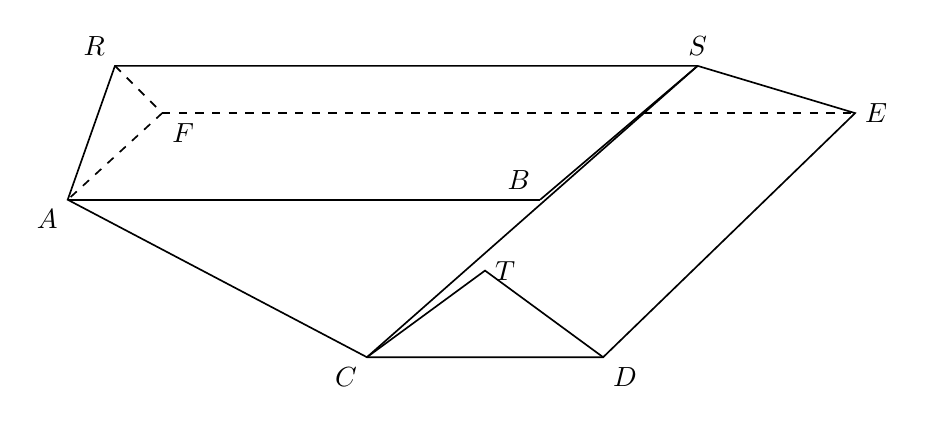
\begin{tikzpicture}[>=stealth,line width=0.6pt,font=\normalsize]
  \coordinate (A) at (0,0);
  \coordinate (R) at (0.6,1.7);
  \coordinate (F) at (1.2,1.1);

  \coordinate (B) at (6.0,0);
  \coordinate (S) at (8.0,1.7);
  \coordinate (E) at (10.0,1.1);

  \coordinate (C) at (3.8,-2.0);
  \coordinate (D) at (6.8,-2.0);
  \coordinate (T) at (5.3,-0.9);

  % 实线可见边
  \draw (A) -- (R) -- (S) -- (E) -- (D) -- (C) -- cycle;
  \draw (A) -- (B);
  \draw (S) -- (B);
  \draw (S) -- (C);
  \draw (C) -- (T) -- (D);

  % 虚线不可见边
  \draw[dashed] (R) -- (F) -- (A);
  \draw[dashed] (F) -- (E);

  % 顶点标注
  \node[below left] at (A) {$A$};
  \node[above left] at (R) {$R$};
  \node[below right] at (F) {$F$};
  \node[above left] at (B) {$B$};
  \node[above] at (S) {$S$};
  \node[right] at (E) {$E$};
  \node[right] at (T) {$T$};
  \node[below left] at (C) {$C$};
  \node[below right] at (D) {$D$};
\end{tikzpicture}
